\documentclass[paper=a4, parskip=half-, ngerman, fontsize=11pt]{scrreprt}
\usepackage[T1]{fontenc}

\usepackage[ngerman]{babel}
\babelprovide[hyphenrules=ngerman-x-latest]{ngerman}

\usepackage{csquotes}
\usepackage[backend=biber]{biblatex}
\addbibresource{Proseminar.bib}

\usepackage{graphicx}
\usepackage{url}


\begin{document}

% Titelseite
\begin{titlepage}
    \begin{center}
        % Unilogo oben
        
\includegraphics[width=0.5\textwidth]{logo_fernuni_hagen.png}\\[2cm]

        {\LARGE \textbf{Übertragung von Signalen auf elektrischen Leitungen}}\\[2cm]

        \textbf{Proseminar Mathematik in der Technik}\\
        \textbf{Modulnummer:} 61711\\
        Fakultät für Mathematik + Informatik\\[0.5cm]

        \begin{tabbing}
            \hspace{6cm} \= \kill
            \textbf{Name:} \> Sven Schmidt \\
            \textbf{Matrikelnummer:} \> 4125169 \\
            \textbf{Abgabedatum:} \> \today \\
            \textbf{Prüfer:} \> PD Dr.-Ing. Stefan Helfert \\
        \end{tabbing}

        \vfill

        {\large FernUniversität in Hagen}\\
        {\large Sommersemester 2025}
    \end{center}
\end{titlepage}

\chapter{Einführung}

\chapter{Modell des Zweidrahtleiters}

In dieser Ausarbeitung beschränken wir uns auf die Untersuchung der Ausbreitung elektromagnetischer Wellen in
Zweidrahtleitern (Paralleldraht), die schematisch in der folgenden Abbildung gezeigt.
\begin{figure}[!h]
    \begin{center}
        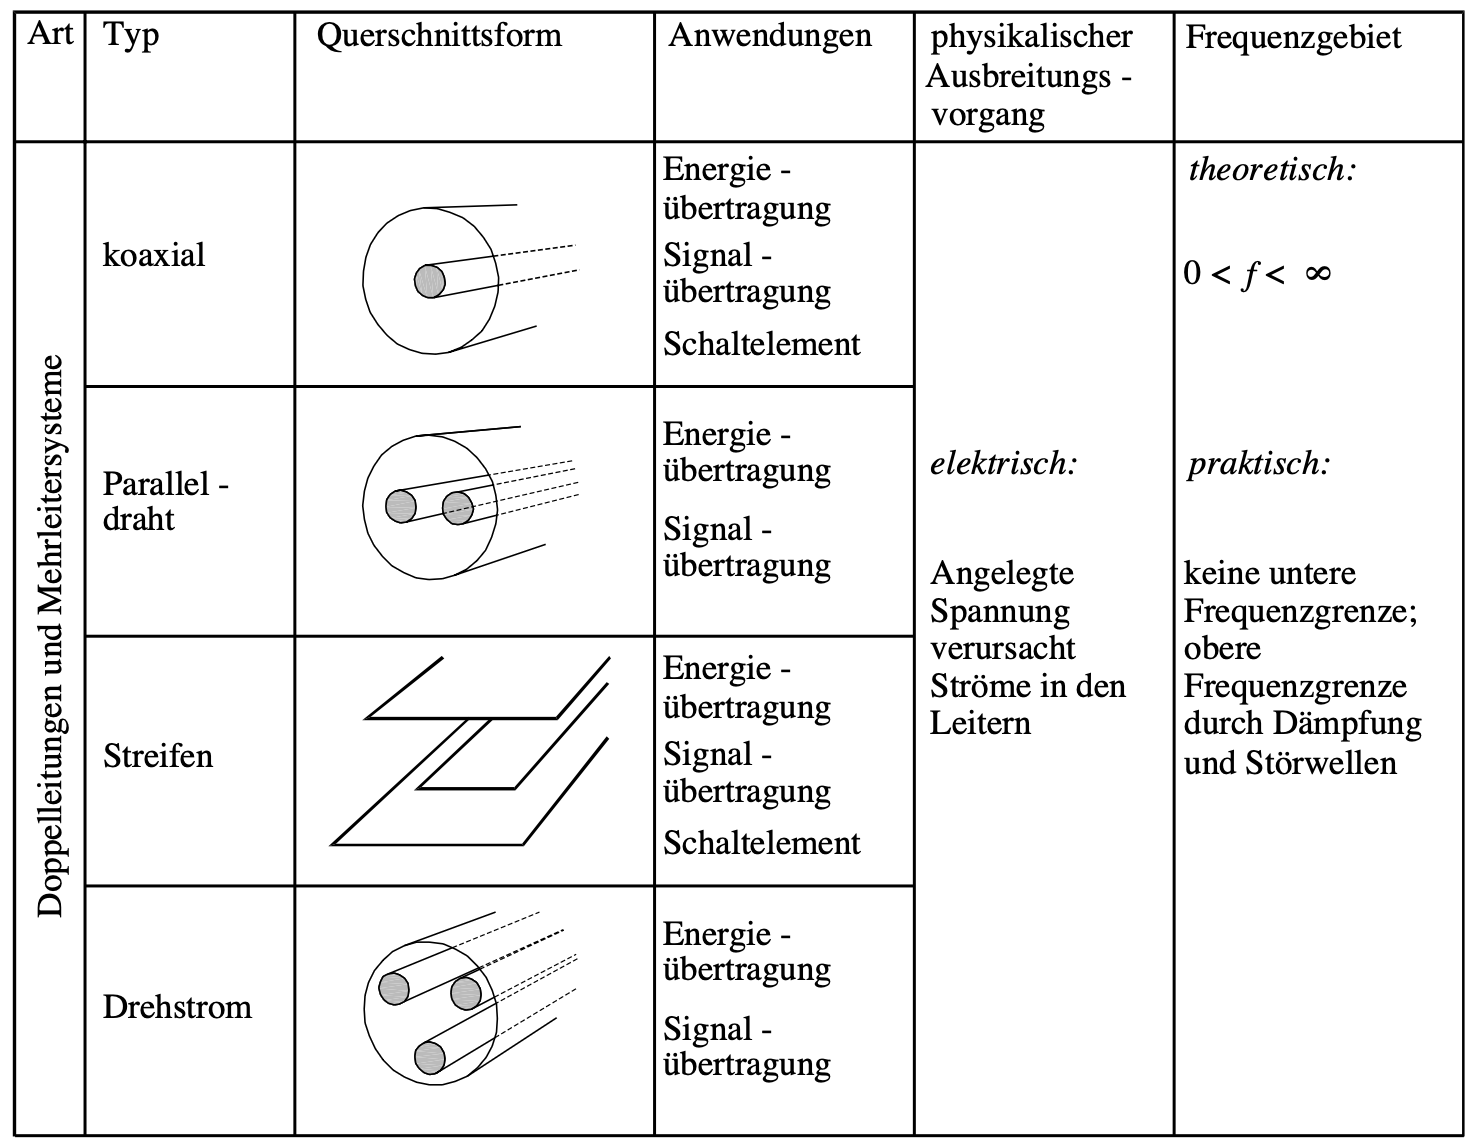
\includegraphics[width=0.5\textwidth]{images/Leiter.png}
        \caption{Elektrische Leiter mit ihren Anwendungen. Entnommen aus~\cite{FernuniSkript}.}
        \label{Leiter}
    \end{center}
\end{figure}

Aus den Gesetzen der Elektro- und Magnetostatik ist bekannt, dass sich beim Durchfließen eines elektrischen Stroms um
den Leiter ein magnetisches Feld ausbildet. Analog bildet die Potenzialdifferenz beider Leiter ein elektrisches Feld
aus. Die folgende Abbildung~\ref{Felder} zeigt den Querschnitt eines Leiters mit eingezeichneten Feldlinien.


\begin{figure}[!h]
    \begin{center}
        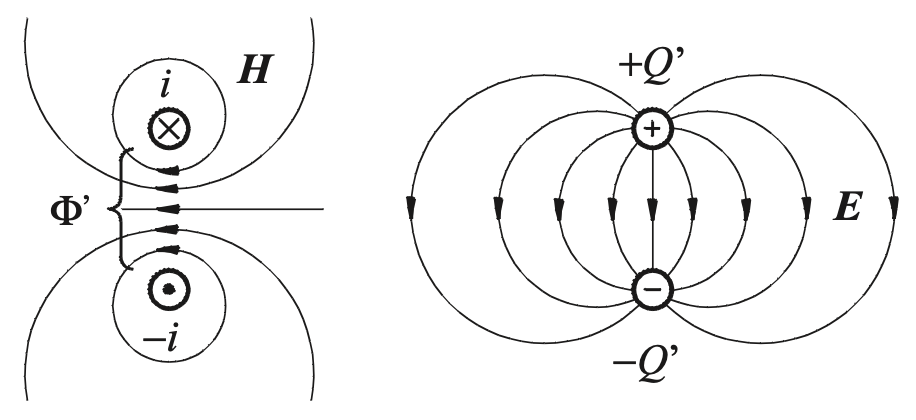
\includegraphics[width=0.5\textwidth]{images/Felder.png}
        \caption{Elektrische Leiter mit ihren Anwendungen. Entnommen aus~\cite{LeitungenUndFilter}.}
        \label{Felder}
    \end{center}
\end{figure}







\chapter{Telegraphenleitungen}

\section{Verlustloses Model}

\section{Verlustbehaftetest Model}

\section{Abschlüsse}


%\bibliographystyle{plain} % oder ein anderer Stil, z.B. alpha, abbrv, unsrt
%\bibliography{Proseminar} % Name Ihrer .bib-Datei OHNE Endung .bib
\printbibliography

\end{document}